\documentclass[../main.tex]{subfiles}

\begin{document}
	\section{Grundlagen}
	
	\subsection{Hosting}
	Unser Produkt soll auf dem neusten Stand der Dinge sein und daher verzichten wir auf den Hoster \gls{hosttech} der schon für das bestehende System verwendet wird. Ein grosser Nachteil von \gls{hosttech} ist das wir auf ein \gls{php} Backend beschränkt sind. Um auch das \gls{deployment} zu modernisieren und hauptsächlich zu automatisieren möchten wir mit \gls{docker} \gls{container} arbeiten. Hierbei hat unser Betreuer Matthias Bachmann seine Plattform angeboten. Auf dieser können wir ein Image des \gls{docker} \gls{container}s hosten lassen. Somit ist dieses zu jederzeit erreichbar. Dies gilt für das Frontend sowie für das Backend.
	Damit der Server nach der Umsetzung nach wie vor erreichbar ist, wurde uns von Matthias Bachmann folgende Seite vorgeschlagen: https://www.hetzner.com/de/
	
	\subsection{Backend Technologie}
	Mit dem Loslösen von \gls{hosttech} sind wir frei die Backend Technologie zu bestimmen und wir haben uns auf \gls{springboot} geeinigt. Wir haben uns für \gls{springboot} entschieden, da alle Entwickler mit Java vertraut sind und \gls{openapi} \gls{springboot} unterstützt. \gls{springboot} eignet sich auch gut für unsere Aufgabenstellung, da wir eine Datenbank anschliessen werden und die Daten auf der Webseite nicht nur dargestellt werden sondern auch manipuliert werden können, eignet sich \gls{springboot} mit der einfachen Handhabung von \gls{jpa} gut.
	
	\subsection{Schnittstelle}
	Als Schnittstelle zwischen Backend und Frontend wollen wir das State of the Art Tool \gls{openapi} einsetzen. Nach genauerer Analyse sehen wir einen grossen Nutzen des Tools, da es uns eine grosse Unterstützung zur Entwicklung der \gls{rest} Schnittstelle sein wird. In \gls{openapi} kann in einem \gls{yaml} File die ganze \gls{rest} Schnittstelle erstellt und konfiguriert werden daraus kann dann \gls{openapi} unser \gls{springboot} Backend erzeugen was uns viel Arbeit abnimmt.
	
	\subsection{Frontend Technologie}
	Das Frontend-Framework können wir frei wählen, da es keine Voraussetzung vom Kunden gab.
	Wir als Gruppe haben uns für \gls{angular}(2+) aus mehreren Gründen entschieden. \\
	\\
	Zum Einen kennt sich die Mehrheit der Gruppe gut mit dem Framework aus, dadurch fällt der Einstieg etwas leichter. Zum Anderen ist die Verwendung von guten Templates in \gls{angular} einfach und effizient. Die Benutzung von einem Template und Komponenten, welche übersichtlich und flexibel verwendet werden können, war für uns ein ausschlaggebender Punkt. \\ 
	Aus diesen Gründen kam \gls{angular} für uns an 1. Stelle zur Sprache.
	
	
	\subsection{Datenbank}
	Um den alten Stand weiterzuführen, wird weiterhin die \gls{mysql} Datenbank benutzt. Diese wird mithilfe der Schnittstelle angepasst.
	Die bestehende Datenbank auf \gls{hosttech} wird in einen neuen \gls{docker} \gls{container} migriert und neben dem \gls{springboot} Projekt gehostet. Nur das \gls{springboot} Projekt hat direkten Zugriff auf die Datenbank, alle Änderungen müssen über die \gls{rest} Schnittstelle der \gls{springboot} Applikation erfolgen.
	
	\begin{figure}[H]
		\centering
		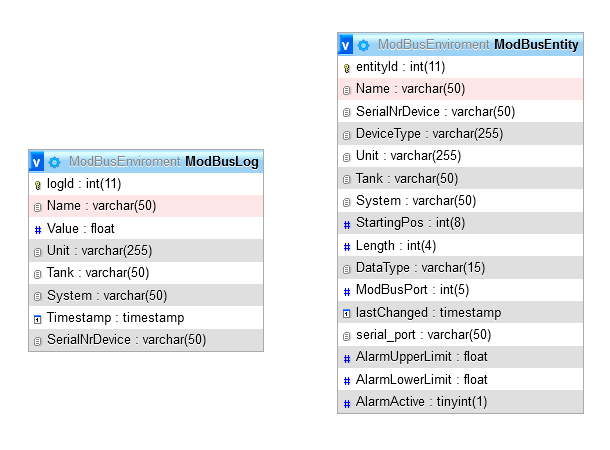
\includegraphics[scale=0.8]{datenbank_overview}
		\caption{Datenbank Überblick}
		\label{fig:datenbank_overview}
	\end{figure}
	\par
	\noindent
	Nach Analyse der Datenbank sahen wir ebenfalls Potential für Verbesserungen, doch wollten wir nicht zu viel an der Struktur ändern, da diese Änderungen weitere Anpassungen auf Systemen erfordern, welche wir keinen Einfluss nehmen können, daher haben wir uns entschieden die Datenbank zu belassen und eine 1 zu 1 Kopie zu erstellen.
\end{document}